
\section{Experiments}
\label{sec:exp}
\subsection{Implementation Details}


We use DA3-Giant~\citep{lin2025depth} fine-tuned on Track4World~\citep{lu2026track4world} as the backbone. We insert a 12-layer causal predictor with width $d_g=1024$ at layer $L_s=12$, where alternating attention begins. For the task instruction, we extract language tokens using a frozen T5 encoder~\citep{raffel2020exploring}. The policy uses a context horizon of $H=4$ for pre-training and $H=1$ for post-training and predicts $C=8$ step action chunks in a $d_a=7$ end-effector action space from $d_s=7$ proprioceptive states. We pretrain GAM on 784K single-arm robot trajectories from RoboCasa365~\citep{nasiriany2026robocasa365}, MimicGen~\citep{mandlekar2023mimicgen}, and OpenX-Embodiment~\citep{collaboration2023open}, then post-train it on each benchmark. We optimize with AdamW using a constant learning rate, freeze layers before $L_s$ and the depth head, and supervise depth with simulator ground truth. We set $\lambda_{\text{act}}=3$, $\lambda_{\text{feat}}=1$, and $\lambda_{\text{depth}}=3$. Further details are provided in the appendix.


\subsection{Experimental Setup}
\label{sec:exp:setup}


\noindent\textbf{Simulation Benchmarks.}
We evaluate generalization across distinct axes using two simulation benchmarks. Specifically, we train our policy on \textbf{LIBERO}~\citep{liu2023libero}, a lifelong single-arm manipulation benchmark spanning diverse spatial layouts, object identities, and task goals. To rigorously assess out-of-distribution robustness, we then evaluate the trained models in a zero-shot manner on \textbf{LIBERO-Plus}~\citep{fei2025libero}, which introduces controlled environmental perturbations across dimensions such as camera viewpoint, lighting, and backgrounds. We report additional results in the appendix.


\definecolor{rankone}{RGB}{255,220,220}   % light red
\definecolor{ranktwo}{RGB}{255,235,200}   % light orange
\definecolor{rankthree}{RGB}{255,250,200} % light yellow

\newcommand{\drop}[1]{{\scriptsize\,($\downarrow$#1)}}

\begin{table*}[t]
\centering
% \scriptsize
% \setlength{\tabcolsep}{3pt}
% \renewcommand{\arraystretch}{0.98}

\caption{\textbf{Evaluation results on LIBERO and LIBERO-Plus.} Success rates are reported in \% with absolute performance drops from LIBERO to LIBERO-Plus shown in parentheses. Color highlights denote the top three performing methods within each column: \colorbox{rankone}{first}, \colorbox{ranktwo}{second}, and \colorbox{rankthree}{third}.}
\label{tab:sim}

\resizebox{\textwidth}{!}{%
\begin{tabular}{@{}l|c|cc|rrrrrrr}
\toprule
Method & Size & Orig. & Plus & Cam. & Robot & Lang. & Light & BG & Noise & Layout \\
\midrule

\multicolumn{11}{c}{\textit{VLAs}} \\
\midrule
$\pi_{0.5}$~\citep{pi05} & 3.3B
& 96.9
& \cellcolor{ranktwo}84.6\drop{12.3}
& \cellcolor{rankthree}72.0
& \cellcolor{rankone}76.6
& \cellcolor{ranktwo}86.5
& \cellcolor{rankthree}96.1
& \cellcolor{rankone}95.2
& \cellcolor{rankthree}86.7
& \cellcolor{rankone}86.0 \\

OpenVLA-OFT~\cite{openvla_oft} & 7B
& 97.1 & 69.6\drop{27.5}
& 56.4 & 31.9 & 79.5 & 88.7
& \cellcolor{rankthree}93.3
& 75.8 & 74.3 \\

RIPT-VLA~\cite{riptvla} & 7B
& 97.5 & 68.4\drop{29.1}
& 55.2 & 31.2 & 77.6 & 88.4
& 91.6
& 73.5 & 74.2 \\

$\pi_0$~\cite{wang2025pi} & 3.3B
& 91.3 & 69.3\drop{22.0}
& 61.0 & 40.8 & 63.7 & 89.3 & 84.1 & 80.1 & 75.9 \\

$\pi_0$-FAST~\cite{pi0_fast} & 3.3B
& 85.5 & 61.6\drop{23.9}
& 65.1 & 21.6 & 61.0 & 73.2 & 73.3 & 74.4 & 68.8 \\

UniVLA~\cite{univla} & 8.5B
& 95.2 & 42.9\drop{52.3}
& 1.8 & 46.2 & 69.5 & 69.0 & 81.0 & 21.2 & 31.9 \\

NORA~\cite{nora} & 3B
& 87.9 & 39.0\drop{48.9}
& 2.2 & 37.0 & 65.1 & 45.7 & 58.6 & 12.8 & 62.1 \\

OpenVLA~\citep{kim2024openvla} & 7B
& 76.5 & 15.6\drop{60.9}
& 0.8 & 3.5 & 23.0 & 8.1 & 34.8 & 15.2 & 28.5 \\

\midrule
\multicolumn{11}{c}{\textit{WAMs}} \\
\midrule
Cosmos-Policy~\citep{kim2026cosmos} & 2B
& \cellcolor{rankone}98.5
& \cellcolor{rankthree}82.4\drop{16.1}
& \cellcolor{ranktwo}73.4
& \cellcolor{rankthree}63.3
& \cellcolor{rankone}89.3
& \cellcolor{rankone}98.9
& 83.5
& \cellcolor{ranktwo}89.3
& \cellcolor{ranktwo}84.0 \\

Fast-WAM~\citep{yuan2026fast} & 6B
& \cellcolor{ranktwo}97.6 & 50.0\drop{47.5}
& 16.4 & 44.5 & 68.9 & 78.2 & 53.7 & 37.7 & 60.7 \\

WorldVLA~\cite{worldvla} & 7B
& 79.1 & 25.0\drop{54.1}
& 0.1 & 27.9 & 41.6 & 43.7 & 17.1 & 11.0 & 38.0 \\



\midrule
\multicolumn{11}{c}{\textit{Geometry-aware VLAs}} \\
\midrule
$\pi_{0.5}$ + Spatial Forcing~\cite{li2025spatial} & 3.3B
& 94.0 & 25.7\drop{58.3}
& 0.1 & 0.3 & 26.8 & 66.0 & 45.9 & 0.1 & 59.8 \\

$\pi_{0.5}$ + ROCKET~\cite{sun2026rocket} & 3.3B
& 95.3 & 47.5\drop{46.6}
& 30.9
& 75.6
& 29.3 & 69.2 & 47.0 & 25.4 & 62.0 \\

\midrule
\multicolumn{11}{c}{\textit{GAM}} \\
\midrule
\textbf{GAM (Ours)} & 1.4B
& \cellcolor{ranktwo}97.6
& \cellcolor{rankone}85.5\drop{12.1}
& \cellcolor{rankone}83.1
& \cellcolor{ranktwo}70.0
& \cellcolor{rankthree}84.8
& \cellcolor{ranktwo}97.2
& \cellcolor{ranktwo}94.3
& \cellcolor{rankone}95.3
& \cellcolor{rankthree}79.1 \\
\bottomrule
\end{tabular}%
}

\vspace{-10pt}
\end{table*}


\noindent\textbf{Real-Robot Setup.}
We train on four manipulation tasks ($\sim$200 demonstrations each) using wrist-mounted and third-person cameras, adhering to the simulation protocol. Since ground-truth geometry is unavailable in the real world, target future depth maps are obtained as pseudo-labels directly from the pretrained backbone GFM. We evaluate robustness via 20 trials per task, divided equally between nominal setups and perturbed environments, specifically varying external camera positions. See the appendix for robot environment with full task and evaluation details.


\noindent\textbf{Baselines.}
We compare GAM against representative baselines from three families discussed in §\ref{sec:related}: \textbf{VLAs}~\citep{kim2024openvla, openvla_oft, black2024pi_0, pi05, pi0_fast, nora, univla, riptvla}, \textbf{WAMs}~\citep{kim2026cosmos, worldvla, yuan2026fast}, and \textbf{geometry-aware VLAs}~\citep{li2025spatial, sun2026rocket}. For the real-robot setup, we compare against $\pi_{0.5}$~\cite{pi05} and Spatial Forcing~\cite{li2025spatial}. For fairness, comparisons utilize a matched evaluation protocol, with performance numbers either re-evaluated using available checkpoints or taken directly from their respective published benchmarks.

\subsection{Main Results}
\label{sec:exp:main}

\noindent\textbf{Simulation Results.} As shown in Table~\ref{tab:sim}, GAM achieves highly competitive success rates on the standard LIBERO benchmark, where performance is heavily saturated. Crucially, on the more challenging LIBERO-Plus benchmark, our model consistently outperforms competing baselines, demonstrating a remarkable improvement in the \textbf{camera-perturbation setting ($\uparrow$9.7\%p)}. This gain highlights the advantage of our end-to-end integration of the GFM. While existing geometry-aware VLAs only partially exploit GFM representations, GAM embeds the GFM throughout its entire predictive pathway to yield a deeply geometry-aware policy.


\noindent\textbf{Real-world Results.} 
To examine whether the gains observed in simulation transfer to physical execution, we additionally evaluate GAM in a real-world setting. Figure~\ref{fig:real_world_eval} shows that GAM substantially outperforms all baselines. In particular, our model remains robust under out-of-domain conditions (the camera-perturbation setting) where other baselines struggle. These results demonstrate that GAM generalizes to the real-world domain and is robust under perturbations, owing to its thorough exploitation of the GFM when training the policy.


\subsection{Ablation Study}
\label{sec:exp:ablation}


\paragraph{Post-training Component Analysis.}
Table~\ref{tab:loss_h_ablation} summarizes ablation study of key post-training components on Object suite of LIBERO and LIBERO-Plus. Pretraining is crucial for robustness: omitting it mildly affects nominal LIBERO but severely degrades LIBERO-Plus. With a pretrained backbone, removing $L_{\text{depth}}$ or $L_{\text{feat}}$ has minimal impact, suggesting geometric dynamics are already encoded.
Notably, even without pretraining, these future-prediction losses provide strong geometric supervision and substantially improve robustness on LIBERO-Plus. Finally, the horizon ablation shows that $H=1$ is sufficient and more robust than longer histories, consistent with prior observations that extended context can introduce spurious correlations~\cite{wen2020fighting,de2019causal}.



\newcommand{\cmark}{\textcolor{green!60!black}{\ding{51}}}
\renewcommand{\xmark}{\textcolor{red!75!black}{\ding{55}}}


\begin{wraptable}[12]{r}{0.66\textwidth}
\centering
\small
\renewcommand{\arraystretch}{0.96}
\vspace{-0.3em} % 주변 텍스트와의 상단 간격

% --- 좌측 열: Table 3 (크기를 살짝 키움) ---
\begin{minipage}[t]{0.56\linewidth}
\centering
\captionof{table}{\textbf{Component ablation.}}
\label{tab:loss_h_ablation}
\vspace{-0.55em}
\resizebox{1.02\linewidth}{!}{% % 1.02로 기본보다 살짝 확대
\begin{tabular}{@{}cccccc@{}}
\toprule
Pretrain & $\mathcal{L}_{\text{depth}}$ & $\mathcal{L}_{\text{feat}}$ & H &
\begin{tabular}{@{}c@{}}Orig.\\SR (\%)\end{tabular} &
\begin{tabular}{@{}c@{}}Plus\\SR (\%)\end{tabular} \\
\midrule
\cmark & \cmark & \cmark & 1 & \textbf{99.6} & \textbf{89.7}\\
\midrule
\cmark & \cmark & \cmark & 2 & 97.2 & 84.4 \\
\cmark & \cmark & \cmark & 4 & 98.2 & 85.1 \\
\midrule
\cmark & \xmark & \cmark & 1 & 98.4 & 89.0 \\
\cmark & \xmark & \xmark & 1 & 98.6 & 89.5 \\
\cmark & \cmark & \xmark & 1 & \textbf{99.6} & \textbf{89.7} \\
\midrule
\xmark & \cmark & \cmark & 1 & 98.4 & 73.4 \\
\xmark & \xmark & \cmark & 1 & 95.2 & 66.5 \\
\xmark & \cmark & \xmark & 1 & 96.4 & 80.0 \\
\xmark & \xmark & \xmark & 1 & 93.6 & 50.0 \\
\bottomrule
\end{tabular}%
}
\end{minipage}%
\hfill
% --- 우측 열: Table 4 & Table 5 (각각 크기를 줄여 높이를 맞춤) ---
\begin{minipage}[t]{0.41\linewidth}
\centering

% [상단] Table 4: Layer ablation (축소 및 캡션 줄바꿈 방지)
\captionof{table}{\textbf{Layer ablation.}}
\label{tab:predictor_layer_ablation}
\vspace{-0.65em}
{% <-- 1. Table 4에만 설정을 제한하기 위한 그룹 시작
\setlength{\tabcolsep}{2.7pt}%
\resizebox{0.85\linewidth}{!}{% % 0.88로 축소하여 세로 높이를 줄임
\begin{tabular}{@{}ccc@{}}
\toprule
Split layer $L_s$  & Orig. (\%)& Plus (\%) \\
\midrule
0  & 5.4 & 1.8 \\
12 & \textbf{99.6} & \textbf{70.1} \\
19 & 95.6 & 63.4 \\
27 & 1.2 & 1.6 \\
33 & 0.0 & 0.0 \\
39 & 0.0 & 0.0 \\
\bottomrule
\end{tabular}%
}}

\vspace{-0.25em} % 우측 두 표 사이의 간격을 좁혀 전체 높이를 튜닝

% [하단] Table 5: Inference efficiency (축소)
\captionof{table}{\textbf{Inference cost.}}
\label{tab:inference_time}
\vspace{0.15em}
\resizebox{0.95\linewidth}{!}{%
\begin{tabular}{@{}lcc@{}}
\toprule
Method & Size & Time \\
\midrule
OpenVLA-OFT~\cite{kim2024openvla}     & 7B   & 77.8ms \\
$\pi_{0.5}$~\cite{pi05}               & 3.3B & 29.2ms   \\
Cosmos-Policy~\cite{kim2026cosmos}    & 2B   & 382.4ms  \\
\textbf{GAM (Ours)}                                  & \textbf{1.4B} & \textbf{6.9ms} \\
\bottomrule
\end{tabular}%
    }
\end{minipage}

\vspace{-1em} % 주변 텍스트와의 하단 간격
\end{wraptable}



\noindent\textbf{Split Layer $L_s$ Selection.}
Table~\ref{tab:predictor_layer_ablation} evaluates the depth of future predictor by shifting the split layer $L_s$ and re-initializing the predictor. We exclude future-depth loss in this experiment because it is not equally applicable to all split layers and could isolate the effect of $\mathcal{L}_{\text{feat}}$ itself. Our default choice of $L_s=12$ achieves peak performance, validating it as the optimal seam between frame-wise and cross-view attention. While layer 19 remains competitive, inserting the predictor too early ($L_s=0$) or late ($L_s\in\{27,33,39\}$) causes total performance collapse. This confirms that forecasted tokens require sufficient interaction through deep layers to properly integrate into the pretrained 3D geometric prior.


\begin{figure*}[t]
    \centering
    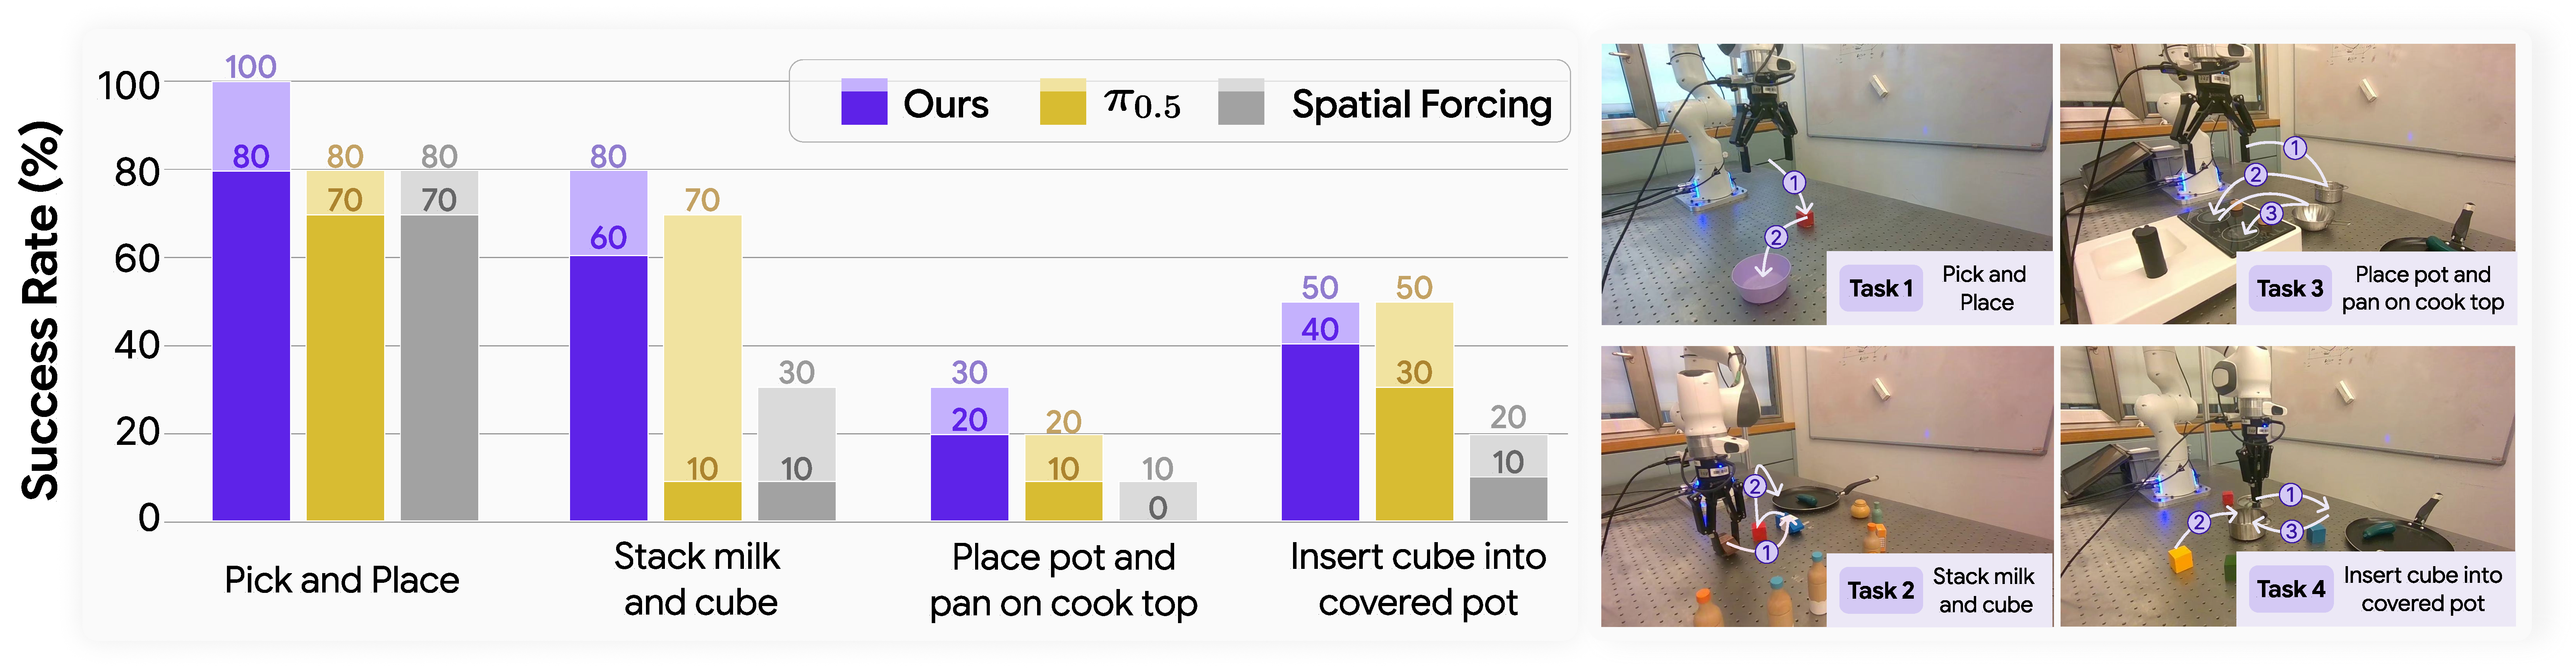
\includegraphics[width=\textwidth]{figures/real_task.pdf}
    \vspace{-15pt}
    \caption{
    \textbf{Real-world robot tasks and results.}
    Each task is evaluated under both in-domain (Light bar) and out-of-domain (Dark bar) settings. The illustration of each task is shown on the right.
    }
    \label{fig:real_world_eval}
    \vspace{-10pt}
\end{figure*}

\subsection{Analysis}
\label{sec:exp:analysis}


\begin{wrapfigure}[11]{r}{0.32\textwidth}
    \centering
    \vspace{-18pt}
    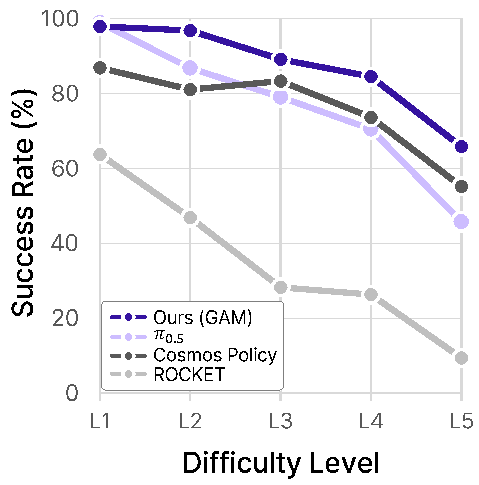
\includegraphics[width=0.9\linewidth]{figures/camera_perturb.pdf}
    \vspace{-5pt}
    \caption{\textbf{Success rate vs.\ camera perturbation difficulty.}}
    \label{fig:camera_perturb}
\end{wrapfigure}
\textbf{Inference Speed and Model Size.}
As shown in Table~\ref{tab:inference_time}, GAM achieves the lowest latency among all baselines, requiring only \textbf{6.9\,ms ($\approx$145\,Hz)} for a single feed-forward pass and running up to 55$\times$ faster than the diffusion-based Cosmos Policy. 
 
All methods are benchmarked under the same setup, with further details provided in the appendix. By utilizing single-pass prediction, GAM avoids the multi-step denoising of diffusion policies, achieving low latency while matching prior accuracy and robustness with only 1.4B parameters.


\noindent\textbf{Robustness to Viewpoint and Scene Variation.} Figure~\ref{fig:camera_perturb} further breaks down the camera-perturbation results by difficulty level of LIBERO-Plus~\cite{fei2025libero}. GAM achieves consistently higher success rates than all baselines at every level, and the advantage remains clear even under the strongest perturbations.
